% Exam Template for UMTYMP and Math Department courses
%
% Using Philip Hirschhorn's exam.cls: http://www-math.mit.edu/~psh/#ExamCls
%
% run pdflatex on a finished exam at least three times to do the grading table on front page.
%
%%%%%%%%%%%%%%%%%%%%%%%%%%%%%%%%%%%%%%%%%%%%%%%%%%%%%%%%%%%%%%%%%%%%%%%%%%%%%%%%%%%%%%%%%%%%%%

% These lines can probably stay unchanged, although you can remove the last
% two packages if you're not making pictures with tikz.
\documentclass[11pt]{exam}
\RequirePackage{amssymb, amsfonts, amsmath, amsthm,latexsym, verbatim, xspace, setspace}
\RequirePackage{tikz, pgflibraryplotmarks}
\usepackage[export]{adjustbox}
% By default LaTeX uses large margins.  This doesn't work well on exams; problems
% end up in the "middle" of the page, reducing the amount of space for students
% to work on them.
\usepackage[margin=1in]{geometry}


% Here's where you edit the Class, Exam, Date, etc.
\newcommand{\class}{Math 1271 - Lectures 010 and 030 }
\newcommand{\term}{Fall 2017}
\newcommand{\examnum}{Quiz 8C}
\newcommand{\examdate}{11/07/17}
\newcommand{\timelimit}{25 Minutes}

% For an exam, single spacing is most appropriate
\singlespacing
% \onehalfspacing
% \doublespacing

% For an exam, we generally want to turn off paragraph indentation
\parindent 0ex

\begin{document} 

% These commands set up the running header on the top of the exam pages
\pagestyle{head}
\firstpageheader{}{}{}
\runningheader{\class}{\examnum\ - Page \thepage\ of \numpages}{\examdate}
\runningheadrule

\begin{flushright}
\begin{tabular}{p{2.8in} r l}
\textbf{\class} & \textbf{Name (Print):} & \makebox[2in]{\hrulefill}\\
\textbf{\term} &&\\
\textbf{\examnum} &&\\
\textbf{\examdate} &&\\
\textbf{Time Limit: \timelimit} & Teaching Assistant & \makebox[2in]{\hrulefill}
\end{tabular}\\
\end{flushright}
\rule[1ex]{\textwidth}{.1pt}

You may \textit{not} use your books, notes, graphing calculator, phones or any other internet devices on this exam.\\

You are required to show your work on each problem on this quiz.  
\begin{minipage}[t]{2.3in}
\vspace{0pt}
%\cellwidth{3em}
\gradetablestretch{2}
\vqword{Problem}
\addpoints % required here by exam.cls, even though questions haven't started yet.	
\gradetable[v]%[pages]  % Use [pages] to have grading table by page instead of question

\end{minipage}
%\newpage % End of cover page

%%%%%%%%%%%%%%%%%%%%%%%%%%%%%%%%%%%%%%%%%%%%%%%%%%%%%%%%%%%%%%%%%%%%%%%%%%%%%%%%%%%%%
%
% See http://www-math.mit.edu/~psh/#ExamCls for full documentation, but the questions
% below give an idea of how to write questions [with parts] and have the points
% tracked automatically on the cover page.
%
%
%%%%%%%%%%%%%%%%%%%%%%%%%%%%%%%%%%%%%%%%%%%%%%%%%%%%%%%%%%%%%%%%%%%%%%%%%%%%%%%%%%%%%
\vskip30mm

\begin{questions}

% Basic question
\addpoints
\question[3] Starting with the initial guess $x_1=-2$, use Newton's method to approximate a root to the equation $e^x+x^2-3=0$ to eight decimal places.
\begin{proof}[Answer]
	$$x_{n+1}=x_n-\frac{f(x_n)}{f'(x_{n})}=x_n-\frac{e^{x_n}+{x_n}^2-3}{e^{x_n}+2{x_n}}$$
	\begin{align*}
	x_1&=-2.00000000\\x_2&= -1.70622671\\x_3&= -1.67751675\\x_4&= -1.67723274\\x_5&= -1.67723271\\ x_6&=
	-1.67723271
	\end{align*}
\end{proof}
% Question with parts
\newpage
\addpoints
\question[4] 
If $600\pi$ cm${}^2$ material is available to make a cylinder with an open top, find the largest possible volume of the cylinder.\newline
Hint: The surface area of a cylinder with an open top is $\pi r^2+2 \pi r h$, where $r$ is the base radius, $h$ is the height.
\begin{figure}[h!]
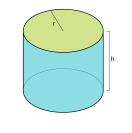
\includegraphics[right]{cyldiag}
\end{figure}
\begin{proof}[Answer]
	\noindent$V=\pi r^2h$\newline
	$A=600\pi=\pi r^2+2\pi r h$
	Solving the above for $h$, we find $$h=\frac{600-r^2}{2r}$$
	Then, \begin{align*}V(r)&=\pi r^2\left(\frac{600-r^2}{2r}\right)\\
	&=300\pi r-\frac{\pi}{2}r^3\\
	\implies V'(r)&=300\pi-\frac{3\pi}{2}r^2\end{align*}
	We note that the endpoints $r=0$ and $h=0$ are physically absurd and the derivative exists everywhere, so the maximum \emph{must} be a critical point of type derivative=0. We find that:\begin{align*}
		0&=300\pi-\frac{3\pi}{2}r_{\max}^2\\
		&=\frac{2}{3\pi}300\pi-r_{\max}^2\\
		&=200-r_{\max}^2\\
		\implies r_\max&=\pm \sqrt{200}=\pm10\sqrt{2}
	\end{align*}
	We note that negative radius is physically absurd and conclude $r_{\max}=10\sqrt{2}$. Then, \begin{align*}h_\max&=\frac{600-r_{\max}^2}{2r_{\max}}\\&=\frac{600-(10\sqrt{2})^2}{20\sqrt{2}}=\frac{600-200}{2\sqrt{200}}=\sqrt{200}=10\sqrt{2}\end{align*}
	cool. great. rad. Putting it together, $V=\pi r^2h=\pi(10\sqrt{2})^3=2000\sqrt{2}\pi$cm${}^2$.
\end{proof}
\vskip70mm
\addpoints
\question[3] Show that the curve $y=\sqrt{x^2+5}+2x$ has one slant asymptote at $y = 3x$ and one horizontal asymptote at $y = 0$.
%\noaddpoints
\begin{proof}[Answer]
Slant asymptote: we notice immediately that $y$ grows without bound as $x$ grows without bound. Thus, the slant asymptote must be on the right. Hence, we take the following limit:
\begin{align*}
	\lim_{x\to\infty}\left((\sqrt{x^2+5}+2x)-3x\right)&=\lim_{x\to\infty}\left((\sqrt{x^2+5}-x)\frac{\sqrt{x^2+5}+x}{\sqrt{x^2+5}+x}\right)\\
	&=\lim_{x\to\infty}\frac{x^2+5-x^2}{\sqrt{x^2+5}+x}\\
	&=\lim_{x\to\infty}\frac{5}{\sqrt{x^2+5}+x}\\&=\lim_{x\to\infty}\frac{5/x}{\sqrt{1+5/x^2}+1}=0
\end{align*}
By process of elimination, the horizontal asymptote must be on the left:
\begin{align*}
	\lim_{x\to-\infty}(\sqrt{x^2+5}+2x)&=	\lim_{x\to-\infty}\left((\sqrt{x^2+5}+2x)\frac{\sqrt{x^2+5}-2x}{\sqrt{x^2+5}-2x}\right)
\end{align*}
Oh! Wait a minute! This problem is false! there isn't a horizontal asymptote, it's a slant asymptote at $y=x$! I'll let you know what the implications for grading are later\textellipsis
\end{proof}
%\addpoints


\end{questions}
\end{document}